
%% bare_jrnl.tex
%% V1.4b
%% 2015/08/26
%% by Michael Shell
%% see http://www.michaelshell.org/
%% for current contact information.
%%
%% This is a skeleton file demonstrating the use of IEEEtran.cls
%% (requires IEEEtran.cls version 1.8b or later) with an IEEE
%% journal paper.
%%
%% Support sites:
%% http://www.michaelshell.org/tex/ieeetran/
%% http://www.ctan.org/pkg/ieeetran
%% and
%% http://www.ieee.org/

%%*************************************************************************
%% Legal Notice:
%% This code is offered as-is without any warranty either expressed or
%% implied; without even the implied warranty of MERCHANTABILITY or
%% FITNESS FOR A PARTICULAR PURPOSE! 
%% User assumes all risk.
%% In no event shall the IEEE or any contributor to this code be liable for
%% any damages or losses, including, but not limited to, incidental,
%% consequential, or any other damages, resulting from the use or misuse
%% of any information contained here.
%%
%% All comments are the opinions of their respective authors and are not
%% necessarily endorsed by the IEEE.
%%
%% This work is distributed under the LaTeX Project Public License (LPPL)
%% ( http://www.latex-project.org/ ) version 1.3, and may be freely used,
%% distributed and modified. A copy of the LPPL, version 1.3, is included
%% in the base LaTeX documentation of all distributions of LaTeX released
%% 2003/12/01 or later.
%% Retain all contribution notices and credits.
%% ** Modified files should be clearly indicated as such, including  **
%% ** renaming them and changing author support contact information. **
%%*************************************************************************


% *** Authors should verify (and, if needed, correct) their LaTeX system  ***
% *** with the testflow diagnostic prior to trusting their LaTeX platform ***
% *** with production work. The IEEE's font choices and paper sizes can   ***
% *** trigger bugs that do not appear when using other class files.       ***                          ***
% The testflow support page is at:
% http://www.michaelshell.org/tex/testflow/



\documentclass[journal]{IEEEtran}
%
% If IEEEtran.cls has not been installed into the LaTeX system files,
% manually specify the path to it like:
% \documentclass[journal]{../sty/IEEEtran}





% Some very useful LaTeX packages include:
% (uncomment the ones you want to load)


% *** MISC UTILITY PACKAGES ***
%
%\usepackage{ifpdf}
% Heiko Oberdiek's ifpdf.sty is very useful if you need conditional
% compilation based on whether the output is pdf or dvi.
% usage:
% \ifpdf
%   % pdf code
% \else
%   % dvi code
% \fi
% The latest version of ifpdf.sty can be obtained from:
% http://www.ctan.org/pkg/ifpdf
% Also, note that IEEEtran.cls V1.7 and later provides a builtin
% \ifCLASSINFOpdf conditional that works the same way.
% When switching from latex to pdflatex and vice-versa, the compiler may
% have to be run twice to clear warning/error messages.






% *** CITATION PACKAGES ***
%
%\usepackage{cite}
% cite.sty was written by Donald Arseneau
% V1.6 and later of IEEEtran pre-defines the format of the cite.sty package
% \cite{} output to follow that of the IEEE. Loading the cite package will
% result in citation numbers being automatically sorted and properly
% "compressed/ranged". e.g., [1], [9], [2], [7], [5], [6] without using
% cite.sty will become [1], [2], [5]--[7], [9] using cite.sty. cite.sty's
% \cite will automatically add leading space, if needed. Use cite.sty's
% noadjust option (cite.sty V3.8 and later) if you want to turn this off
% such as if a citation ever needs to be enclosed in parenthesis.
% cite.sty is already installed on most LaTeX systems. Be sure and use
% version 5.0 (2009-03-20) and later if using hyperref.sty.
% The latest version can be obtained at:
% http://www.ctan.org/pkg/cite
% The documentation is contained in the cite.sty file itself.






% *** GRAPHICS RELATED PACKAGES ***
%
\usepackage{pgfplots}

\ifCLASSINFOpdf
  %\usepackage[pdftex]{graphicx}
  % declare the path(s) where your graphic files are
  %\graphicspath{{img/}}
  % and their extensions so you won't have to specify these with
  % every instance of \includegraphics
  %\DeclareGraphicsExtensions{.jpg,.pdf,.jpeg,.png}
\else
  % or other class option (dvipsone, dvipdf, if not using dvips). graphicx
  % will default to the driver specified in the system graphics.cfg if no
  % driver is specified.
  % \usepackage[dvips]{graphicx}
  % declare the path(s) where your graphic files are
  % \graphicspath{{../eps/}}
  % and their extensions so you won't have to specify these with
  % every instance of \includegraphics
  % \DeclareGraphicsExtensions{.eps}
\fi
% graphicx was written by David Carlisle and Sebastian Rahtz. It is
% required if you want graphics, photos, etc. graphicx.sty is already
% installed on most LaTeX systems. The latest version and documentation
% can be obtained at: 
% http://www.ctan.org/pkg/graphicx
% Another good source of documentation is "Using Imported Graphics in
% LaTeX2e" by Keith Reckdahl which can be found at:
% http://www.ctan.org/pkg/epslatex
%
% latex, and pdflatex in dvi mode, support graphics in encapsulated
% postscript (.eps) format. pdflatex in pdf mode supports graphics
% in .pdf, .jpeg, .png and .mps (metapost) formats. Users should ensure
% that all non-photo figures use a vector format (.eps, .pdf, .mps) and
% not a bitmapped formats (.jpeg, .png). The IEEE frowns on bitmapped formats
% which can result in "jaggedy"/blurry rendering of lines and letters as
% well as large increases in file sizes.
%
% You can find documentation about the pdfTeX application at:
% http://www.tug.org/applications/pdftex





% *** MATH PACKAGES ***
%
%\usepackage{amsmath}
% A popular package from the American Mathematical Society that provides
% many useful and powerful commands for dealing with mathematics.
%
% Note that the amsmath package sets \interdisplaylinepenalty to 10000
% thus preventing page breaks from occurring within multiline equations. Use:
%\interdisplaylinepenalty=2500
% after loading amsmath to restore such page breaks as IEEEtran.cls normally
% does. amsmath.sty is already installed on most LaTeX systems. The latest
% version and documentation can be obtained at:
% http://www.ctan.org/pkg/amsmath





% *** SPECIALIZED LIST PACKAGES ***
%
%\usepackage{algorithmic}
% algorithmic.sty was written by Peter Williams and Rogerio Brito.
% This package provides an algorithmic environment fo describing algorithms.
% You can use the algorithmic environment in-text or within a figure
% environment to provide for a floating algorithm. Do NOT use the algorithm
% floating environment provided by algorithm.sty (by the same authors) or
% algorithm2e.sty (by Christophe Fiorio) as the IEEE does not use dedicated
% algorithm float types and packages that provide these will not provide
% correct IEEE style captions. The latest version and documentation of
% algorithmic.sty can be obtained at:
% http://www.ctan.org/pkg/algorithms
% Also of interest may be the (relatively newer and more customizable)
% algorithmicx.sty package by Szasz Janos:
% http://www.ctan.org/pkg/algorithmicx




% *** ALIGNMENT PACKAGES ***
%
%\usepackage{array}
% Frank Mittelbach's and David Carlisle's array.sty patches and improves
% the standard LaTeX2e array and tabular environments to provide better
% appearance and additional user controls. As the default LaTeX2e table
% generation code is lacking to the point of almost being broken with
% respect to the quality of the end results, all users are strongly
% advised to use an enhanced (at the very least that provided by array.sty)
% set of table tools. array.sty is already installed on most systems. The
% latest version and documentation can be obtained at:
% http://www.ctan.org/pkg/array


% IEEEtran contains the IEEEeqnarray family of commands that can be used to
% generate multiline equations as well as matrices, tables, etc., of high
% quality.




% *** SUBFIGURE PACKAGES ***
%\ifCLASSOPTIONcompsoc
%  \usepackage[caption=false,font=normalsize,labelfont=sf,textfont=sf]{subfig}
%\else
%  \usepackage[caption=false,font=footnotesize]{subfig}
%\fi
% subfig.sty, written by Steven Douglas Cochran, is the modern replacement
% for subfigure.sty, the latter of which is no longer maintained and is
% incompatible with some LaTeX packages including fixltx2e. However,
% subfig.sty requires and automatically loads Axel Sommerfeldt's caption.sty
% which will override IEEEtran.cls' handling of captions and this will result
% in non-IEEE style figure/table captions. To prevent this problem, be sure
% and invoke subfig.sty's "caption=false" package option (available since
% subfig.sty version 1.3, 2005/06/28) as this is will preserve IEEEtran.cls
% handling of captions.
% Note that the Computer Society format requires a larger sans serif font
% than the serif footnote size font used in traditional IEEE formatting
% and thus the need to invoke different subfig.sty package options depending
% on whether compsoc mode has been enabled.
%
% The latest version and documentation of subfig.sty can be obtained at:
% http://www.ctan.org/pkg/subfig




% *** FLOAT PACKAGES ***
%
%\usepackage{fixltx2e}
% fixltx2e, the successor to the earlier fix2col.sty, was written by
% Frank Mittelbach and David Carlisle. This package corrects a few problems
% in the LaTeX2e kernel, the most notable of which is that in current
% LaTeX2e releases, the ordering of single and double column floats is not
% guaranteed to be preserved. Thus, an unpatched LaTeX2e can allow a
% single column figure to be placed prior to an earlier double column
% figure.
% Be aware that LaTeX2e kernels dated 2015 and later have fixltx2e.sty's
% corrections already built into the system in which case a warning will
% be issued if an attempt is made to load fixltx2e.sty as it is no longer
% needed.
% The latest version and documentation can be found at:
% http://www.ctan.org/pkg/fixltx2e


%\usepackage{stfloats}
% stfloats.sty was written by Sigitas Tolusis. This package gives LaTeX2e
% the ability to do double column floats at the bottom of the page as well
% as the top. (e.g., "\begin{figure*}[!b]" is not normally possible in
% LaTeX2e). It also provides a command:
%\fnbelowfloat
% to enable the placement of footnotes below bottom floats (the standard
% LaTeX2e kernel puts them above bottom floats). This is an invasive package
% which rewrites many portions of the LaTeX2e float routines. It may not work
% with other packages that modify the LaTeX2e float routines. The latest
% version and documentation can be obtained at:
% http://www.ctan.org/pkg/stfloats
% Do not use the stfloats baselinefloat ability as the IEEE does not allow
% \baselineskip to stretch. Authors submitting work to the IEEE should note
% that the IEEE rarely uses double column equations and that authors should try
% to avoid such use. Do not be tempted to use the cuted.sty or midfloat.sty
% packages (also by Sigitas Tolusis) as the IEEE does not format its papers in
% such ways.
% Do not attempt to use stfloats with fixltx2e as they are incompatible.
% Instead, use Morten Hogholm'a dblfloatfix which combines the features
% of both fixltx2e and stfloats:
%
% \usepackage{dblfloatfix}
% The latest version can be found at:
% http://www.ctan.org/pkg/dblfloatfix




%\ifCLASSOPTIONcaptionsoff
%  \usepackage[nomarkers]{endfloat}
% \let\MYoriglatexcaption\caption
% \renewcommand{\caption}[2][\relax]{\MYoriglatexcaption[#2]{#2}}
%\fi
% endfloat.sty was written by James Darrell McCauley, Jeff Goldberg and 
% Axel Sommerfeldt. This package may be useful when used in conjunction with 
% IEEEtran.cls'  captionsoff option. Some IEEE journals/societies require that
% submissions have lists of figures/tables at the end of the paper and that
% figures/tables without any captions are placed on a page by themselves at
% the end of the document. If needed, the draftcls IEEEtran class option or
% \CLASSINPUTbaselinestretch interface can be used to increase the line
% spacing as well. Be sure and use the nomarkers option of endfloat to
% prevent endfloat from "marking" where the figures would have been placed
% in the text. The two hack lines of code above are a slight modification of
% that suggested by in the endfloat docs (section 8.4.1) to ensure that
% the full captions always appear in the list of figures/tables - even if
% the user used the short optional argument of \caption[]{}.
% IEEE papers do not typically make use of \caption[]'s optional argument,
% so this should not be an issue. A similar trick can be used to disable
% captions of packages such as subfig.sty that lack options to turn off
% the subcaptions:
% For subfig.sty:
% \let\MYorigsubfloat\subfloat
% \renewcommand{\subfloat}[2][\relax]{\MYorigsubfloat[]{#2}}
% However, the above trick will not work if both optional arguments of
% the \subfloat command are used. Furthermore, there needs to be a
% description of each subfigure *somewhere* and endfloat does not add
% subfigure captions to its list of figures. Thus, the best approach is to
% avoid the use of subfigure captions (many IEEE journals avoid them anyway)
% and instead reference/explain all the subfigures within the main caption.
% The latest version of endfloat.sty and its documentation can obtained at:
% http://www.ctan.org/pkg/endfloat
%
% The IEEEtran \ifCLASSOPTIONcaptionsoff conditional can also be used
% later in the document, say, to conditionally put the References on a 
% page by themselves.




% *** PDF, URL AND HYPERLINK PACKAGES ***
%
%\usepackage{url}
% url.sty was written by Donald Arseneau. It provides better support for
% handling and breaking URLs. url.sty is already installed on most LaTeX
% systems. The latest version and documentation can be obtained at:
% http://www.ctan.org/pkg/url
% Basically, \url{my_url_here}.




% *** Do not adjust lengths that control margins, column widths, etc. ***
% *** Do not use packages that alter fonts (such as pslatex).         ***
% There should be no need to do such things with IEEEtran.cls V1.6 and later.
% (Unless specifically asked to do so by the journal or conference you plan
% to submit to, of course. )


% correct bad hyphenation here
\hyphenation{op-tical net-works semi-conduc-tor}


% Package for highlighting text. \hl{My text} will highlight "My text"
\usepackage{soul, color}

\begin{document}
%
% paper title
% Titles are generally capitalized except for words such as a, an, and, as,
% at, but, by, for, in, nor, of, on, or, the, to and up, which are usually
% not capitalized unless they are the first or last word of the title.
% Linebreaks \\ can be used within to get better formatting as desired.
% Do not put math or special symbols in the title.
\title{Implementation of a Non-Blocking\\ Hashtable using C++11}
%
%
% author names and IEEE memberships
% note positions of commas and nonbreaking spaces ( ~ ) LaTeX will not break
% a structure at a ~ so this keeps an author's name from being broken across
% two lines.
% use \thanks{} to gain access to the first footnote area
% a separate \thanks must be used for each paragraph as LaTeX2e's \thanks
% was not built to handle multiple paragraphs
%

\author{Timothy~Flowers,
        Austin~Lasher,
        and~Joseph~Maag% <-this % stops a space
}

% note the % following the last \IEEEmembership and also \thanks - 
% these prevent an unwanted space from occurring between the last author name
% and the end of the author line. i.e., if you had this:
% 
% \author{....lastname \thanks{...} \thanks{...} }
%                     ^------------^------------^----Do not want these spaces!
%
% a space would be appended to the last name and could cause every name on that
% line to be shifted left slightly. This is one of those "LaTeX things". For
% instance, "\textbf{A} \textbf{B}" will typeset as "A B" not "AB". To get
% "AB" then you have to do: "\textbf{A}\textbf{B}"
% \thanks is no different in this regard, so shield the last } of each \thanks
% that ends a line with a % and do not let a space in before the next \thanks.
% Spaces after \IEEEmembership other than the last one are OK (and needed) as
% you are supposed to have spaces between the names. For what it is worth,
% this is a minor point as most people would not even notice if the said evil
% space somehow managed to creep in.



% The paper headers
\markboth{UCF COP4520 -- Parallel Processing, Assignment 2}
{Shell \MakeLowercase{\textit{et al.}}: Bare Demo of IEEEtran.cls for IEEE Journals}
% The only time the second header will appear is for the odd numbered pages
% after the title page when using the twoside option.
% 
% *** Note that you probably will NOT want to include the author's ***
% *** name in the headers of peer review papers.                   ***
% You can use \ifCLASSOPTIONpeerreview for conditional compilation here if
% you desire.




% If you want to put a publisher's ID mark on the page you can do it like
% this:
%\IEEEpubid{0000--0000/00\$00.00~\copyright~2015 IEEE}
% Remember, if you use this you must call \IEEEpubidadjcol in the second
% column for its text to clear the IEEEpubid mark.



% use for special paper notices
%\IEEEspecialpapernotice{(Invited Paper)}




% make the title area
\maketitle

% As a general rule, do not put math, special symbols or citations
% in the abstract or keywords.
\begin{abstract}
In the paper “Non-blocking Hashtables with Open Addressing”, Chris Purcell and Tim Harris propose a non-blocking hashtable that utilizes buckets, probe bounds, and open addressing for standard hashtable functionality and achieves non-blocking behavior with the use of atomic operations and custom word types. We implemented a sequential version of the proposed hashtable in a C++11 class that shares the core hashtable implementation but eliminates much of what makes it parallel. Our implementation was tested over a series of trials and resulted in a degradation of performance as the number of of threads performing operations was increased (I hope?).
\end{abstract}

% Note that keywords are not normally used for peerreview papers.
%\begin{IEEEkeywords}
%IEEE, IEEEtran, journal, \LaTeX, paper, template.
%\end{IEEEkeywords}






% For peer review papers, you can put extra information on the cover
% page as needed:
% \ifCLASSOPTIONpeerreview
% \begin{center} \bfseries EDICS Category: 3-BBND \end{center}
% \fi
%
% For peerreview papers, this IEEEtran command inserts a page break and
% creates the second title. It will be ignored for other modes.
%\IEEEpeerreviewmaketitle




\section{Introduction}
% The very first letter is a 2 line initial drop letter followed
% by the rest of the first word in caps.
% 
% form to use if the first word consists of a single letter:
% \IEEEPARstart{A}{demo} file is ....
% 
% form to use if you need the single drop letter followed by
% normal text (unknown if ever used by the IEEE):
% \IEEEPARstart{A}{}demo file is ....
% 
% Some journals put the first two words in caps:
% \IEEEPARstart{T}{his demo} file is ....
% 
% Here we have the typical use of a "T" for an initial drop letter
% and "HIS" in caps to complete the first word.
\IEEEPARstart{I}{n} this paper we will describe a  sequential version of a non-blocking hashtable described by Chris Purcell and Tim Harris in their paper “Non-blocking Hashtables with Open Addressing”. We implemented the data structure a a C++11 class and performed a series of tests to assess its performance.
To describe our implementation and test results, we will first in Section 1 briefly describe the hashtable proposed in the original paper. Section 2 will describe the details of our C++11 sequential implementation of the hashtable. Lastly, we will describe our performance tests and analyze the results to give an overall view of the efficiency of a sequential version of the described hashtable.


% You must have at least 2 lines in the paragraph with the drop letter
% (should never be an issue)
%I wish you the best of success.

%\hfill mds
 
%\hfill August 26, 2015

%\subsection{Subsection Heading Here}
%Subsection text here.

% needed in second column of first page if using \IEEEpubid
%\IEEEpubidadjcol

%\subsubsection{Subsubsection Heading Here}
%Subsubsection text here.


% An example of a floating figure using the graphicx package.
% Note that \label must occur AFTER (or within) \caption.
% For figures, \caption should occur after the \includegraphics.
% Note that IEEEtran v1.7 and later has special internal code that
% is designed to preserve the operation of \label within \caption
% even when the captionsoff option is in effect. However, because
% of issues like this, it may be the safest practice to put all your
% \label just after \caption rather than within \caption{}.
%
% Reminder: the "draftcls" or "draftclsnofoot", not "draft", class
% option should be used if it is desired that the figures are to be
% displayed while in draft mode.
%

% Note that the IEEE typically puts floats only at the top, even when this
% results in a large percentage of a column being occupied by floats.


% An example of a double column floating figure using two subfigures.
% (The subfig.sty package must be loaded for this to work.)
% The subfigure \label commands are set within each subfloat command,
% and the \label for the overall figure must come after \caption.
% \hfil is used as a separator to get equal spacing.
% Watch out that the combined width of all the subfigures on a 
% line do not exceed the text width or a line break will occur.
%
%\begin{figure*}[!t]
%\centering
%\subfloat[Case I]{\includegraphics[width=2.5in]{box}%
%\label{fig_first_case}}
%\hfil
%\subfloat[Case II]{\includegraphics[width=2.5in]{box}%
%\label{fig_second_case}}
%\caption{Simulation results for the network.}
%\label{fig_sim}
%\end{figure*}
%
% Note that often IEEE papers with subfigures do not employ subfigure
% captions (using the optional argument to \subfloat[]), but instead will
% reference/describe all of them (a), (b), etc., within the main caption.
% Be aware that for subfig.sty to generate the (a), (b), etc., subfigure
% labels, the optional argument to \subfloat must be present. If a
% subcaption is not desired, just leave its contents blank,
% e.g., \subfloat[].


% An example of a floating table. Note that, for IEEE style tables, the
% \caption command should come BEFORE the table and, given that table
% captions serve much like titles, are usually capitalized except for words
% such as a, an, and, as, at, but, by, for, in, nor, of, on, or, the, to
% and up, which are usually not capitalized unless they are the first or
% last word of the caption. Table text will default to \footnotesize as
% the IEEE normally uses this smaller font for tables.
% The \label must come after \caption as always.
%
%\begin{table}[!t]
%% increase table row spacing, adjust to taste
%\renewcommand{\arraystretch}{1.3}
% if using array.sty, it might be a good idea to tweak the value of
% \extrarowheight as needed to properly center the text within the cells
%\caption{An Example of a Table}
%\label{table_example}
%\centering
%% Some packages, such as MDW tools, offer better commands for making tables
%% than the plain LaTeX2e tabular which is used here.
%\begin{tabular}{|c||c|}
%\hline
%One & Two\\
%\hline
%Three & Four\\
%\hline
%\end{tabular}
%\end{table}


% Note that the IEEE does not put floats in the very first column
% - or typically anywhere on the first page for that matter. Also,
% in-text middle ("here") positioning is typically not used, but it
% is allowed and encouraged for Computer Society conferences (but
% not Computer Society journals). Most IEEE journals/conferences use
% top floats exclusively. 
% Note that, LaTeX2e, unlike IEEE journals/conferences, places
% footnotes above bottom floats. This can be corrected via the
% \fnbelowfloat command of the stfloats package.


\section{Algorithm Description}

The Non-Blocking implementation of our Hashtable contains three operations: Insert, Delete, and Contains. The function of these operations is described below, as well as a description of the necessary changes for a Non-Blocking implementation.\hl{All in all, this section (below) is far too similar to our ''implementation'' section. This section should have more to do with the algorithm itself, and its parallelization. The implementation section should be our personal considerations and choices in the code we wrote.}

\subsection{Insert}
In order to insert into the table, the hash value must first be obtained. Starting from the bucket corresponding to the hash value, continue quadratic probing until they find a bucket that contains an EMPTY\_FLAG value. If the number of probes to get to that slot was greater than the upper bound stored for the inserted item's hash value, the upper bound should be updated to the number of probe jumps used to reach the EMPTY slot. Otherwise, the probe bound should remain unchanged. If at any point the number of probe jumps exceeds the size of the hash table, the function should return false to signal that the collision was unresolved and the insert operation failed. \hl{More detail would be nice, we should also throw in details about the ideal algorithm, and how it is Non-blocking.}

\subsection{Remove}
In order to remove an element from the table, the hash value for the element must first be obtained. Starting from the bucket corresponding to the hash value, continue probing until the element is found or the upper bounds are exceeded. If the upper bound is exceeded return false to signal that the item was unable to be removed. If the item is found set the bucket its located in to EMPTY. If the number of probe jumps it takes to get to the bucket is equal to the upper bounds of the hash value, decrement the upper bound until probing by the number contained within the upper bound results in a non-empty bucket, or the upper bound equals zero.\hl{Same as above paragraph.}

\subsection{Contains}
In order to check for an element in the table, the hash value must first be obtained. Then starting from the bucket corresponding to the hash value, probing should continue until the upper bound of the hash value is exceeded or until the element to be searched for is found. If the element is found return true. Otherwise, if the bounds are exceeded, return false.


\section{Implementation}

Our C++11 implementation of the sequential hashtable data structure has many similarities to the structure and pseudocode described by Chris Purcell and Tim Harris, but has several changes to keep it sequential while utilizing the features of C++11.

\subsection{C++11}
The structure is encapsulated in a C++ class called NBHashTable with a standard C++ class source file ‘NBHashTable.cpp’ and header file ‘NBHashTable.h’. C++11 was chosen as our implementation language so we could utilize the thread support library that is part of the C++11 standard library. NBHashTable utilizes a ‘std::mutex’ object from the thread library to guarantee thread-safety. ‘std::thread’ objects are used in our main test classes to spawn threads and have them interact with a NBHashTable object.

\subsection{Buckets and Probe Bounds}
The internal storage structure of NBHashTable is an integer array ‘buckets’ that represents the hashtable bucket locations. The size of the array is determined by an integer argument passed into the NBHashTable constructor method. This value is assigned to an internal size variable ‘kSize’ and is used throughout the hashtable class, including for the instantiation of the buckets array. In our current implementation the variable is not constant, which will be necessary for making our hashtable resizable in the future.

Initially the bucket array locations are initialized to the value of the preprocessor macro 'EMPTY\_FLAG' defined in the NBHashTable header file. In our implementation it is set to -1 to represent an empty bucket. It is assumed only integers greater than -1 will be placed into buckets except when a value is removed from a bucket, in which case it is set back to the empty flag value -1.

The bounds values associated with each bucket location are represented as an integer array initialized to be the same size as the buckets array. Each location in the array is initially initialized to 0 to represent 0 collisions at each bucket location.

\subsection{Public Methods}
The public methods to ‘put’ and ‘remove’ values in NBHashTable have arguments of type NBType. NBType is defined in the header file as a typedef integer type. This type is used as an alternative to a standard ‘int’ to make possible changes to this type easier in future development.

Before each addition or removal of an integer value, the value is passed into a hash function to make an associated index that is within the range of this buckets and bounds array. This hash function is simply '(value \% kSize)' where kSize is the hashtable size.

The methods used to interact with the buckets are similar to those described in the paper, with one method to obtain values from the bucket, and one method to test whether a given collision exists. Both take a ‘startIndex’ integer argument representing the hashed version of an integer value to be added or removed, and a ‘probeJumps’ integer representing the length of the probe sequence needed to find the value. A pointer to a bounds location is returned when getting a bucket value so that the value can be changed without having to access the the bucket array twice. While not entirely necessary for our sequential implementation, this will be useful if we need to parallelize NBHashTable in the future.

When inserting or removing a value from the hashtable, the value is first hashed with the has method and is used as the first index location in the buckets array that is checked. When inserting, if there is already a value in that position in the array, other locations in the area are checked to be empty to find a location where it can be inserted instead. The locations checked in this probing sequence are determined by the quadratic formula '(startIndex + (probeJumps * (probeJumps + 1)) / 2'. This probing is executed in a for-loop with a counter called ‘probeJumps’, which is iterated until it is greater than the kSize constant or an empty location is found at an index defined by the quadratic equation.

When removing or locating an item, the same probing sequence is used, except the for-loop stops when the counter is greater than the bounds value at the original hash value location (or when the value it is searching for is found first).

As described in the paper, bound values are incremented with the addition of values whose collision value is greater than the hash indexes original value in the bounds array. A bound value is decremented with the removal of a value last in a probing sequence. The method ’conditionallyLowerBound’ is responsible for calculating and setting a new bounds uses a loop to search the probe sequence in reverse until it reaches a non-empty bucket, and then sets a new probe value at the original hash index.

\subsection{Sequential Modifications}
To keep the algorithm parallel and lock-free, the pseudocode provided uses lock-free atomic compare-and-swap functions when accessing and modifying bucket and bounds values. The paper also specifies packing a state, a version count, and a bucket value into a single word value for each bucket for atomic access and modification. The paper also suggests using a single word value that contains a scanning bit and a bounds value for each bounds value.

These modifications make the structure lock-free and parallel, so our implementation does not use them in order to keep the structure sequential. Bucket and bounds values are simply integer values that represent the bucket value, without any additional state values. Reads and writes to the bounds and buckets arrays are done directly without atomic operations. To keep the structure sequential and thread-safe, we use a single std::mutex object that is locked for every public method call and unlocked at the end of every public method. Even though this allows blocking and eliminates the non-blocking nature of the proposed hashtable, this guarantees only one public method can be executed at a time so that no two threads will be interacting with the hashtable at the same time. If one thread is interacting with the hashtable and another thread attempts to call one of its public methods simultaneously, it will have to wait until the first thread is finished. At this point, the holding thread will unlock the mutex, and a waiting thread will begin its interaction by locking it. Because NBHashTable public methods cannot execute simultaneously, sequential performance is guaranteed.


\section{Testing and Performance}

To compare our algorithm to the original description, we set up several testing suites that implemented our NBHashTable class. We were testing to measure two key properties: correctness, and execution time.

\subsection{Correctness}

Correctness is difficult to measure for all cases. Unlike execution time, it would be difficult to create a testing suite to measure correctness that randomly generates numbers. It would randomly have to generate insertions and deletions of numbers, and from that compare it to a "correct" output, that it would also have to generate. How can we be sure that the output it created was actually correct for every case? There is no way to be sure, as there could be a fault in our procedure that generates a "correct" output. A false positive, in this case, would be likely.

Our approach to measuring the correctness of the algorithm, instead, was to create several test cases. The idea is that we can create test cases, and compare the actual result to an expected result we retrieved on paper. With this method, we can create many different tricky test cases, and see how they perform individually.

We have included our sample test cases in our initial submission document, under ''correctness1.cpp'' and ''correctness2.cpp''. \hl{Write more about this, create more actual test cases.}

\subsection{Execution time}

Execution time is important to test because it allows us to compare the specific operations of the algorithm and determine how it should be used most efficiently. It also allows us to compare our implementation to the expected time from the original paper, and potentially see the limits of our currently sequential solution.



%\includegraphics[width=100px]{kitten}

\hl{More}

%\begin{figure}[!h]
%\centering
%\includegraphics[width=2.5in]{kitten}
%\caption{Trial 1 - 75\% insertion, 25\% deletion, 0\% contains operations.}
%\label{fig_sim}
%\end{figure}


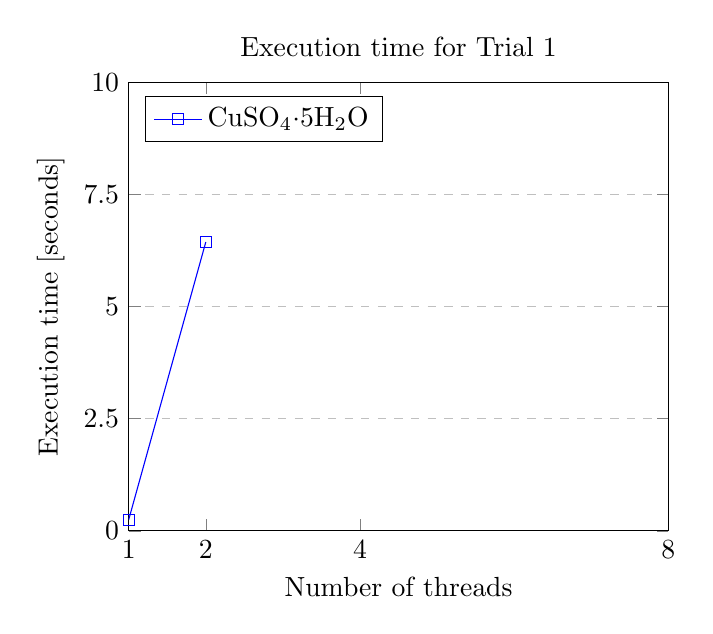
\begin{tikzpicture}
\begin{axis}[
    title={Execution time for Trial 1},
    xlabel={Number of threads},
    ylabel={Execution time [seconds]},
    xmin=1, xmax=8,
    ymin=0, ymax=10,
    xtick={1,2,4,8},
    ytick={0, 2.5, 5, 7.5, 10},
    legend pos=north west,
    ymajorgrids=true,
    grid style=dashed,
]
 
\addplot[
    color=blue,
    mark=square,
    ]
    coordinates {
    %0.2487	6.4415
    (1, 0.2487)(2,6.4415)
    };
    \legend{CuSO$_4\cdot$5H$_2$O}
 
\end{axis}
\end{tikzpicture}


\section{Analysis and Conclusion}

\hl{Here we talk about our results, compare them to the original paper.}
The non-blocking hashtable proposed by Chris Purcell and Tim Harris uses a number of operations and specialized data types to achieve atomicity non-blocking functionality.  To make our implementation sequential, we were able to simplify the internal structure of the hashtable by eliminating these features and only allowing one thread to modify the hashtable at a time. Though this differentiates it from the proposed implementation and is not non-blocking, it maintains the same hashtable open addressing functionality with the use of probe scanning phases. The result is a sequential version of the proposed hashtable structure.


% if have a single appendix:
%\appendix[Proof of the Zonklar Equations]
% or
%\appendix  % for no appendix heading
% do not use \section anymore after \appendix, only \section*
% is possibly needed

% use appendices with more than one appendix
% then use \section to start each appendix
% you must declare a \section before using any
% \subsection or using \label (\appendices by itself
% starts a section numbered zero.)
%


%\appendices
%\section{Proof of the First Zonklar Equation}
%Appendix one text goes here.

% you can choose not to have a title for an appendix
% if you want by leaving the argument blank
%\section{}
%Appendix two text goes here.


% use section* for acknowledgment
%\section*{Acknowledgment}


%The authors would like to thank...


% Can use something like this to put references on a page
% by themselves when using endfloat and the captionsoff option.
\ifCLASSOPTIONcaptionsoff
  \newpage
\fi



% trigger a \newpage just before the given reference
% number - used to balance the columns on the last page
% adjust value as needed - may need to be readjusted if
% the document is modified later
%\IEEEtriggeratref{8}
% The "triggered" command can be changed if desired:
%\IEEEtriggercmd{\enlargethispage{-5in}}

% references section

% can use a bibliography generated by BibTeX as a .bbl file
% BibTeX documentation can be easily obtained at:
% http://mirror.ctan.org/biblio/bibtex/contrib/doc/
% The IEEEtran BibTeX style support page is at:
% http://www.michaelshell.org/tex/ieeetran/bibtex/
%\bibliographystyle{IEEEtran}
% argument is your BibTeX string definitions and bibliography database(s)
%\bibliography{IEEEabrv,../bib/paper}
%
% <OR> manually copy in the resultant .bbl file
% set second argument of \begin to the number of references
% (used to reserve space for the reference number labels box)
\begin{thebibliography}{1}

% Purcell, C., Harris, T.: In: Proceedings of the 19th International Conference on Distributed Computing,
% pp. 108–121. Springer-Verlag, Berlin, Heidelberg, DISC’05 (2005).

\bibitem{IEEEhowto:kopka}

C.~Purcell and T.~Harris, \emph{Non-blocking Hashtables with Open Addressing}.\hskip 1em plus
  0.5em minus 0.4em\relax Springer-Verlag, Berlin, Heidelberg, 2005.

\end{thebibliography}

% biography section
% 
% If you have an EPS/PDF photo (graphicx package needed) extra braces are
% needed around the contents of the optional argument to biography to prevent
% the LaTeX parser from getting confused when it sees the complicated
% \includegraphics command within an optional argument. (You could create
% your own custom macro containing the \includegraphics command to make things
% simpler here.)
%\begin{IEEEbiography}[{\includegraphics[width=1in,height=1.25in,clip,keepaspectratio]{mshell}}]{Michael Shell}
% or if you just want to reserve a space for a photo:

%\begin{IEEEbiography}{Michael Shell}
%Biography text here.
%\end{IEEEbiography}

% if you will not have a photo at all:
%\begin{IEEEbiographynophoto}{John Doe}
%Biography text here.
%\end{IEEEbiographynophoto}

% insert where needed to balance the two columns on the last page with
% biographies
%\newpage

%\begin{IEEEbiographynophoto}{Jane Doe}
%Biography text here.
%\end{IEEEbiographynophoto}

% You can push biographies down or up by placing
% a \vfill before or after them. The appropriate
% use of \vfill depends on what kind of text is
% on the last page and whether or not the columns
% are being equalized.

%\vfill

% Can be used to pull up biographies so that the bottom of the last one
% is flush with the other column.
%\enlargethispage{-5in}



% that's all folks
\end{document}


